\chapter{Problem Solving}%
\label{chap:problem-solving}

\section{Exploiting Fractions for Fun and Profit}
\label{sec:proportions-rates}

\subsection{Absolute and Relative Change}
\label{sub:absolute-relative-change}

In this section we will see how to use the two arithemtic operations
of subtraction and division to measure how something changes over
time.
\begin{definition}
  \textbf{Absolute change} is the difference:
  \[
    \text{absolute change} = \text{new} - \text{old}
  \]
\end{definition}

Absolute change can be useful for comparing things that are similar.
For example you could compare how many inches two fourteen year old
boys grew in one year. But suppose the things you wish to compare are
related but on very different size scales.

\begin{example}[Stock Investments Part I]
  Suppose you invest \$50,000 in Acme corporation stock and after one
  year the stock is now worth \$52,000. This is an absolute change of
  \$2,000. Now suppose you also invest \$500 in Hooli corporation and
  after one year the stock is worth \$550. Which investment was better?
\end{example}
\begin{solution}
  \begin{align*}
    \text{absolute change in Acme} &= \$52,000 - \$50,000 = \$2,000 \\
    \text{absolute change in Hooli} &= \$550 - \$500 = \$50
  \end{align*}
  In terms of absolute change the yield from the Acme investment is
  larger, so it is better right? Well what if we had switched our
  investment strategy and swapped the initial stock purchase for each
  company? To answer this question we need to see how big the absolute
  change in value was relative to the initial outlay of money. We need
  relative change.
\end{solution}

\begin{definition}
  \textbf{Relative change} is the ratio of absolute change to the original (old) value.
  \[
    \text{relative change} = \frac{\text{new} - \text{old}}{\text{old}}
  \]
\end{definition}

\begin{example}[Stock Investments Part II]
What is the relative change in value of each stock purchase?
\end{example}
\begin{solution}
  \begin{align*}
    \text{relative change in Acme}
    &= \frac{\$52,000 - \$50,000}{\$50,000} = \frac{\$2,000}{\$50,000} = 0.04 \\
    \text{relative change in Hooli}
    &= \frac{\$550 - \$500}{\$500} = \frac{\$50}{\$500} = 0.10
  \end{align*}
  Hooli's relative change was higher than Acme's relative change, and
  thus the Hooli stock was the better investment.
\end{solution}

\begin{note}
  Notice that absolute change has units attached to the value. In the
  above examples the units were dollars (\$). But when you compute
  relative change, the numerator and denominator will have the same
  units and thus the units will cancel and you are left with a pure
  (unitless) number.
\end{note}

\subsection{Percentages}
\label{sub:percentages}

\begin{definition}
  A \textbf{percent} or \textbf{percentage} is a fraction, where the
  denominator is 100, but for ease of writing we drop the denominator
  and replace it with the percent symbol \(\%\). For example,
  \[
    \frac{3}{4} = 0.75 = \frac{75}{100} = 75\%
  \]
  Percentages can be negative and even larger than 100, for example
  \[
    250\% = \frac{250}{100} = 2.5
  \]
\end{definition}

\begin{exercise}
  Express the following values as percentages.
  \begin{enumerate}
  \item \(\displaystyle\frac{1}{5}\)
    \vspace*{\stretch{1}}
  \item \(\displaystyle 0.004\)
    \vspace*{\stretch{1}}
  \item \(\displaystyle 3.11\)
    \vspace*{\stretch{1}}
  \end{enumerate}
\end{exercise}

It is often convenient to express relative change as a percent
\begin{example}[Stock Investments Part III]
  What was the percent change in value of each stock investment?
  \begin{center}
    \begin{tabular}{rccc}
      \toprule
      Company & Decimal & Fraction & Percent \\
      \midrule
      Acme & .04 & \(\frac{4}{100}\) & 4\% \\ \\
      Hooli & .10 & \(\frac{10}{100}\) & 10\% \\
      \bottomrule
    \end{tabular}
\end{center}
\end{example}

\newpage

\begin{exercise}
  Your truck was worth \$28,000 in 2019 and is now worth \$23,500 in
  2021. What is the percent change in value of your truck?

  \vspace*{\stretch{1}}
\end{exercise}


\begin{exercise}
  Your \$290,000 home increased in value by 5\%. How much is it worth now?

  \vspace*{\stretch{1}}
\end{exercise}

\begin{exercise}
  A store has a clearance rack where every item is marked down 20\%
  off the original price. They have a sale advertising an additional
  20\% off everything in the store. What percentage of the original
  price do you end up paying?

  \vspace*{\stretch{1}}
\end{exercise}

\newpage

\subsection{Rates}
\label{sub:rates}

\begin{definition}
  A \text{rate} is a ratio of two quantities. Rates are also known as
  fractions.
\end{definition}

\begin{exercise}
  If your car can travel \US{284}{\mile} per fillup and your gas tank
  holds \US{9.5}{\gallon}, then at what rate does your car consume
  gasoline, or more commonly, what is its mpg?

  \vspace*{\stretch{1}}
\end{exercise}

\subsection{Proportionality}
\label{sub:proportionality}

\begin{definition}
  A \text{proportion} is a ratio of two quantities. Thus it is a fraction.
\end{definition}

\begin{exercise}
  A map's legend indicates that \US{0.5}{\inch} equals
  \US{4}{\mile}. How many miles apart in real life are two points on
  the map that are separated by \US{3.5}{\inch}?

  \vspace*{\stretch{1}}
\end{exercise}

\begin{exercise}
  A cookie recipe calls for 2 cups of chocolate chips per batch of 24
  cookies. If you wish to make 216 cookies?

  \vspace*{\stretch{1}}
\end{exercise}

\newpage

\section{Exploiting Units for Fun and Profit}
\label{sec:exploiting-units}

\begin{exercise}
  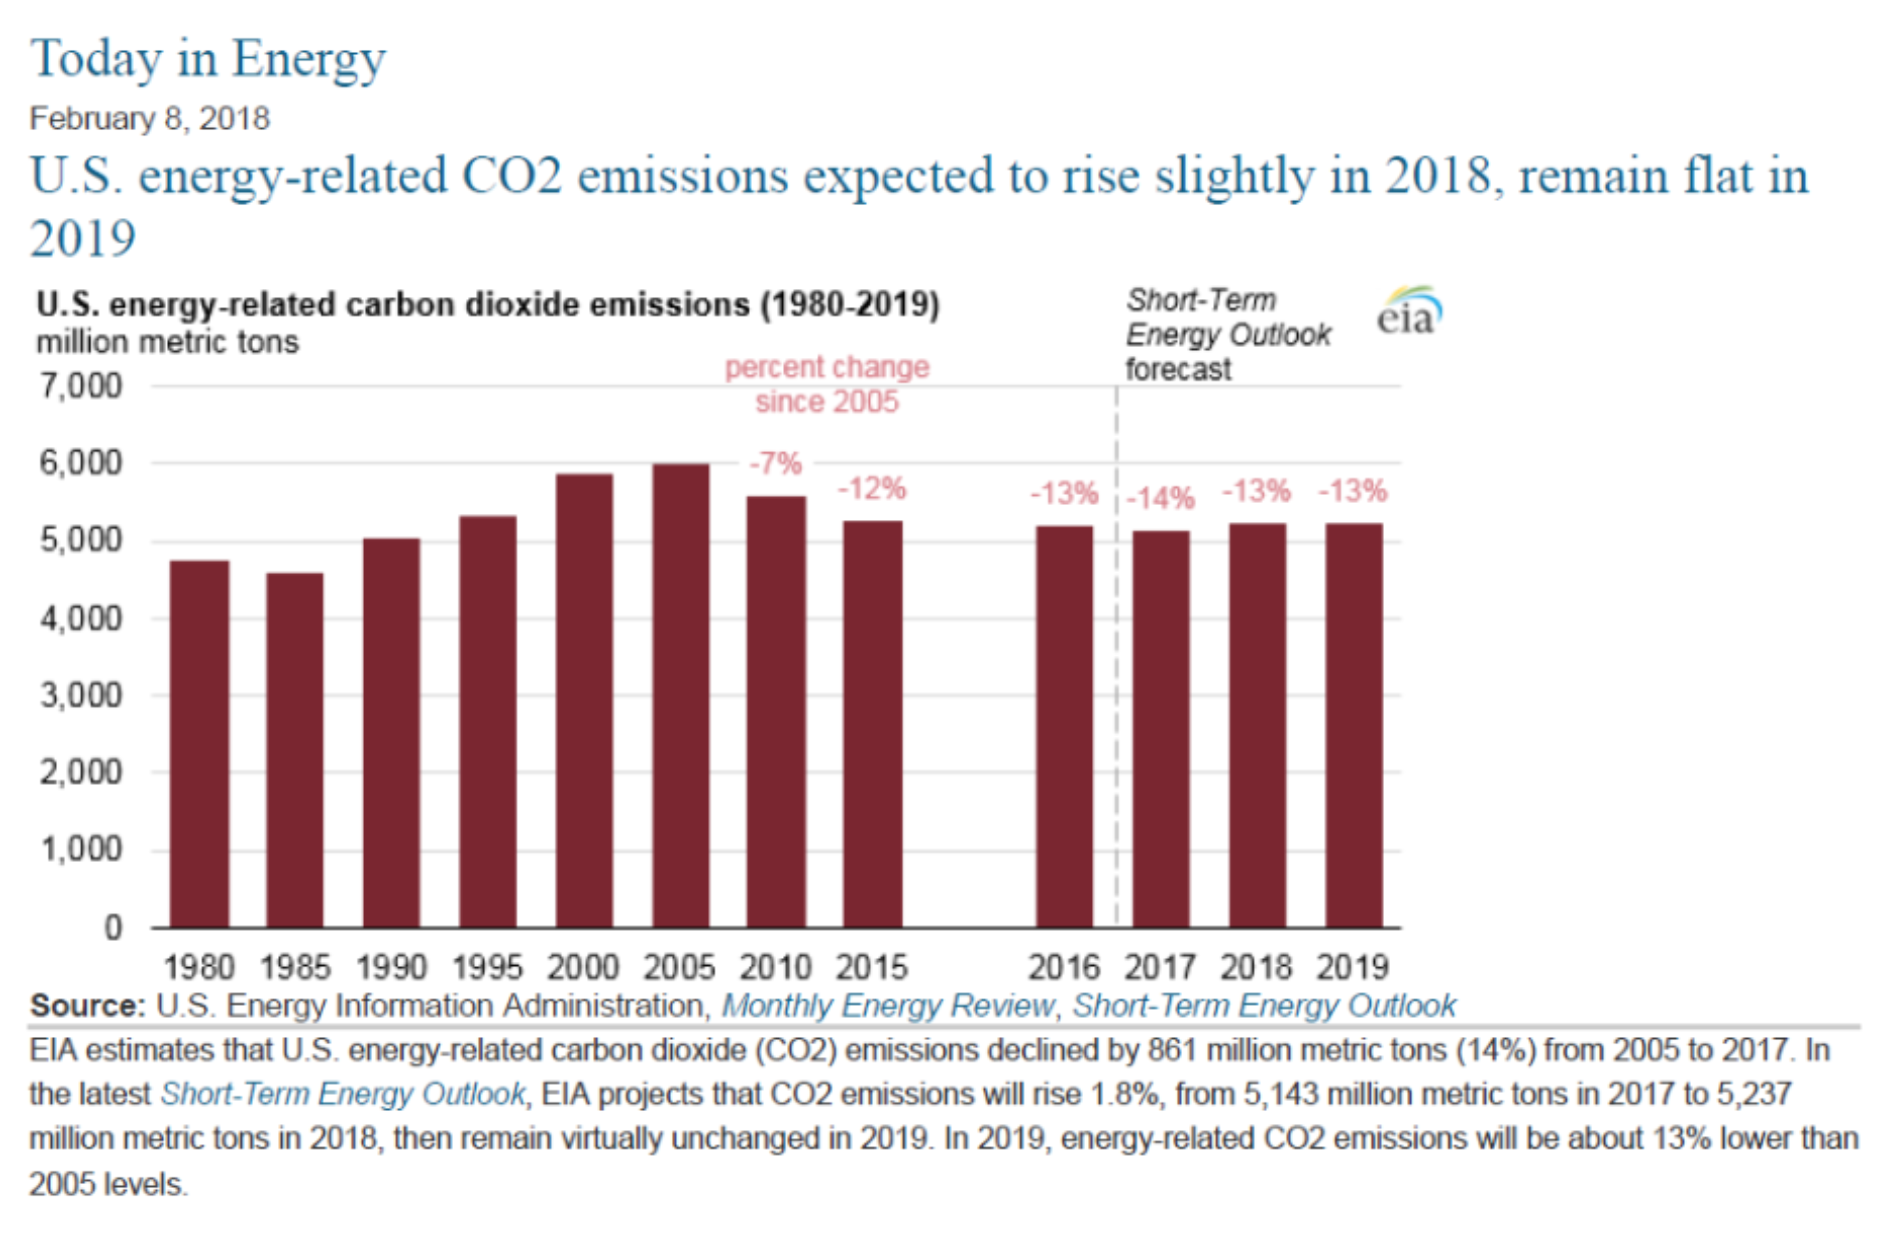
\includegraphics[scale=0.5]{CO2_Emissions}
  \begin{enumerate}
  \item According to EIA how much carbon did the American energy
    sector emit in 2017? How much is it predicted to emit in 2018 and
    2019?

    \vspace*{\stretch{1}}

  \item Use the absolute change from 2005 to 2017 given in the first
    sentence to calculated U.S. energy-related emissions in 2005.

    \vspace*{\stretch{1}}

  \item Use the result from part 2 to calculate the relative change
    from 2005 to 2017. Does your value agree with the given
    percentage?

    \vspace*{\stretch{1}}

    \newpage

    \begin{center}
      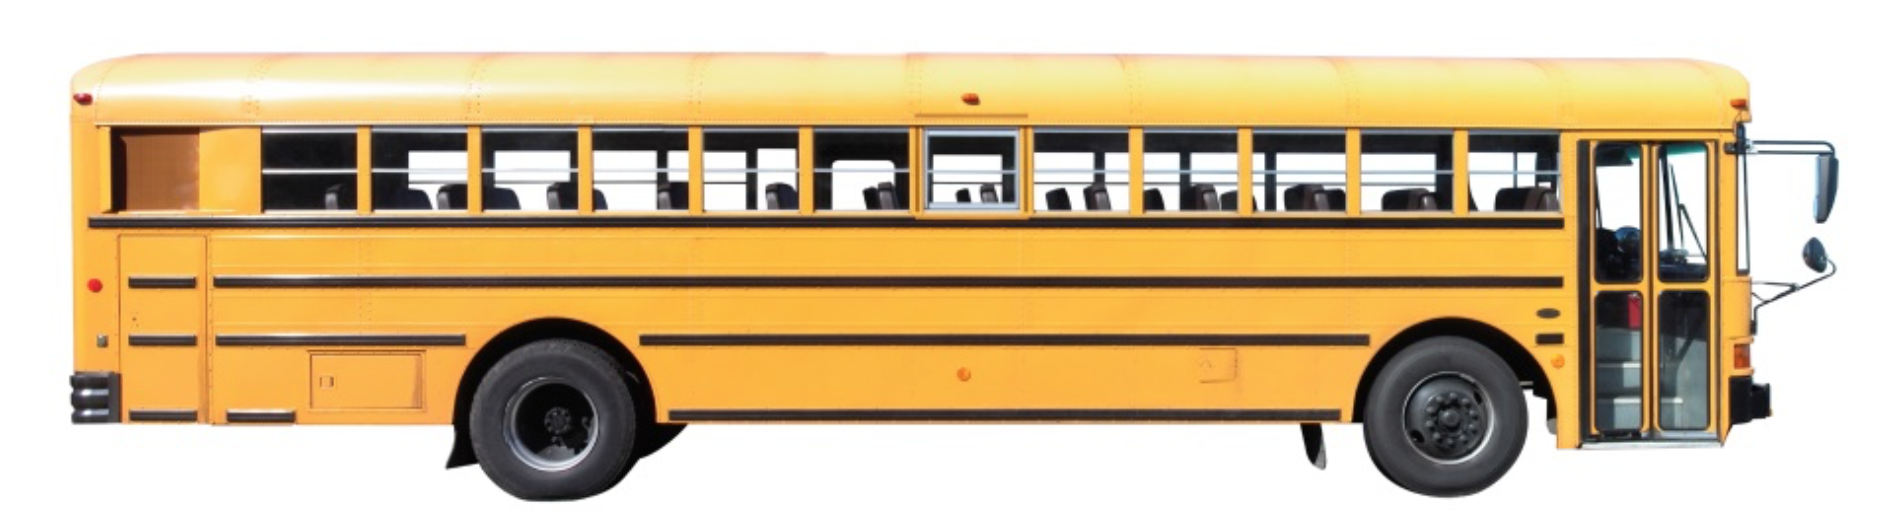
\includegraphics[scale=0.2]{schoolbus}
    \end{center}
  \item A Type D school bus weighs about 15 metric tons. How many
    school buses worth of \(\text{CO}_2\) did the American energy
    industry emit in 2005?
    \vspace*{\stretch{1}}

  \item How many school buses worth of \(\text{CO}_2\) is the American
    energy industry predicted to emit in 2019?

    \vspace*{\stretch{1}}


  \item According to the American School Bus Council about 480,000
    buses are used each day in the United States. Compare the weight
    of all those buses to the weight of the \(\text{CO}_2\) the U.S.
    energy sector is predicted to emit in 2019.

    \vspace*{\stretch{1}}
  \end{enumerate}
\end{exercise}

\newpage

\subsection{Unit Conversions}%
\label{sub:unit-conversions}

\begin{table}[h]
  \centering
  \begin{tabular}{lr@{ = }l}
    \toprule
    Length & 12 in & 1 ft \\
           & 3 ft & 1 yd \\
           & 5280 ft & 1 mi \\
    \midrule
    Weight & 1 lb & 16 oz \\
           & 1 ton & 2000 lb \\
    \midrule
    Capacity & 1 fl oz & \(\tfrac{1}{8}\) cup \\
           & 1 cup & 8 fl oz \\
           & 1 pint & 16 fl oz (2 cups) \\
           & 1 quart & 32 fl oz (4 cups) \\
           & 1 gallon & 128 fl oz (4 quarts) \\
    \bottomrule
  \end{tabular}
  \caption{Common US unit conversions}%
  \label{tab:unit-conversions}
\end{table}

\begin{exercise}
  Convert 5 cubic yards to cubic feet.

  \vspace*{\stretch{1}}
\end{exercise}

\newpage

\begin{exercise}
  During a massive Canadian ice storm, 30 thousand acres of sugarbush
  crop were damaged, where each acre of sugarbush grows about 80
  trees. You can assume that each tree yields \(\tfrac{1}{2}\) gallon
  of maple syrup a year, and Canada typically produces 8 million
  gallons of maple syrup per year.

  \begin{enumerate}
  \item What percentage of the maple syrup supply in Canada was destroyed
    that year?

    \vspace*{\stretch{1}}

  \item If maple syrup is worth \$39.10 per gallon and the average
    farmer tends to 45 acres of sugarbush, how much income did the
    average farmer lose that year?

    \vspace*{\stretch{1}}

  \end{enumerate}
\end{exercise}

\newpage

\begin{figure}[h]
  \centering
  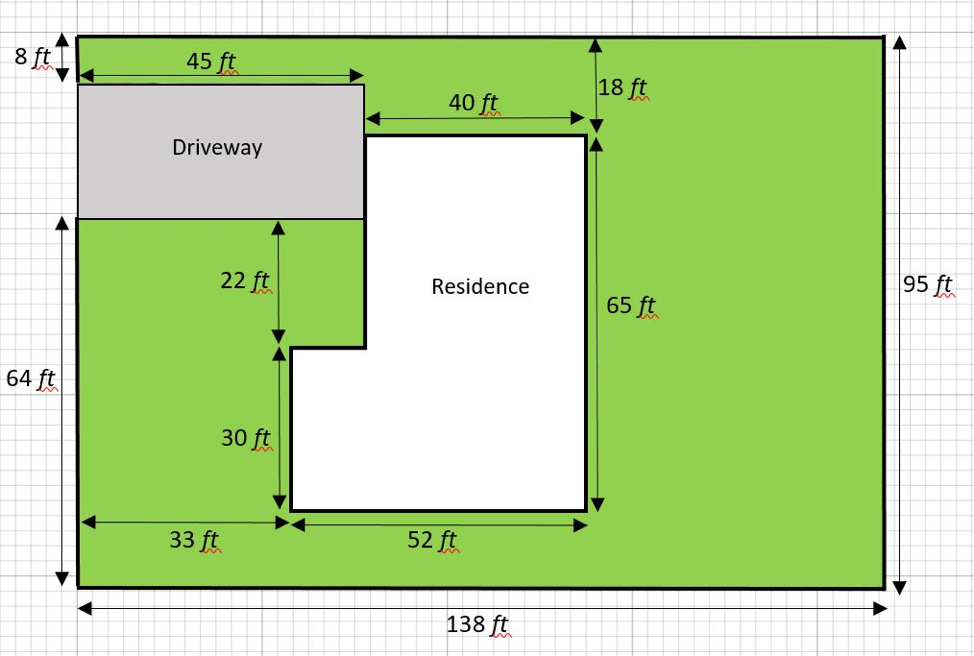
\includegraphics[width=\textwidth]{yard-schematic}
  \caption{Schematic of a plot of land.}%
  \label{fig:yard-schematic}
\end{figure}

\begin{exercise}
  Your neighbor's lawn isn't looking too good. He has decided to
  remove all the old sod (grass), bring in a new 4 inch layer of
  topsoil, install new in-ground sprinklers, and reseed the lawn. He
  seems to think that he'll be able to save money by hauling loads of
  topsoil from the store himself in his pickup truck, rather than
  paying for delivery, but you're not sure he's right. You're going to
  help him.
  \begin{enumerate}
  \item Using Figure~\ref{fig:yard-schematic}, find the area of the
    yard via the following steps:
    \begin{enumerate}
    \item Find the area of the entire lot.

      \vspace*{\stretch{1}}

    \item Find the area of the residence.

      \vspace*{\stretch{1}}

    \item Find the area of the driveway.

      \vspace*{\stretch{1}}

    \item Find the area of the yard.
    \end{enumerate}

    \newpage

  \item We are supposed to put a 4 inch layer of topsoil over the area
    of the yard.

    \begin{enumerate}
    \item Find the required topsoil in cubic feet.

      \vspace*{\stretch{1}}

    \item Convert the required volume of topsoil to cubic yards.

      \vspace*{\stretch{1}}

    \item Find the cost of the topsoil. (\$18 per cubic yard sold in
      \(\tfrac{1}{4}\) cubic yard increments)

      \vspace*{\stretch{1}}
    \end{enumerate}

  \item Suppose we pay \$30 per truckload on top of the soil cost.
    Each truckload can deliver up to 18 cubic yards.
    \begin{enumerate}
    \item How many truckloads are required?

      \vspace*{\stretch{1}}

    \item How much will the delivery cost?

      \vspace*{\stretch{1}}

    \end{enumerate}

    \newpage

  \item Suppose we use the pickup truck. The bed is 80 inches long, 69
    inches wide, and 20 inches tall.
    \begin{enumerate}
    \item Calculate the volume of the pickup in cubic inches.

      \vspace*{\stretch{1}}

    \item Convert the volume of the pickup to cubic yards.

      \vspace*{\stretch{1}}

    \item How many trips to the store will we need to make?

      \vspace*{\stretch{1}}

    \item The store is 9 miles away and it takes 20 minutes to drive
      there. The truck gets 17 miles to the gallon and gasoline costs
      \$3.79 per gallon. How much will we pay to get the soil
      ourselves?

      \vspace*{\stretch{1}}

    \item How much time will we spend driving?
    \end{enumerate}

      \vspace*{\stretch{1}}

  \end{enumerate}
\end{exercise}



% \subsection{Geometry: Area and Volume Formulas}
% \label{sub:geometry}


% \subsection{Linear, Areal and Volumetric Densities}
% \label{sub:densities}





%%% Local Variables:
%%% mode: latex
%%% TeX-master: "Notes"
%%% End:
